\begin{figure}[H]
\centering
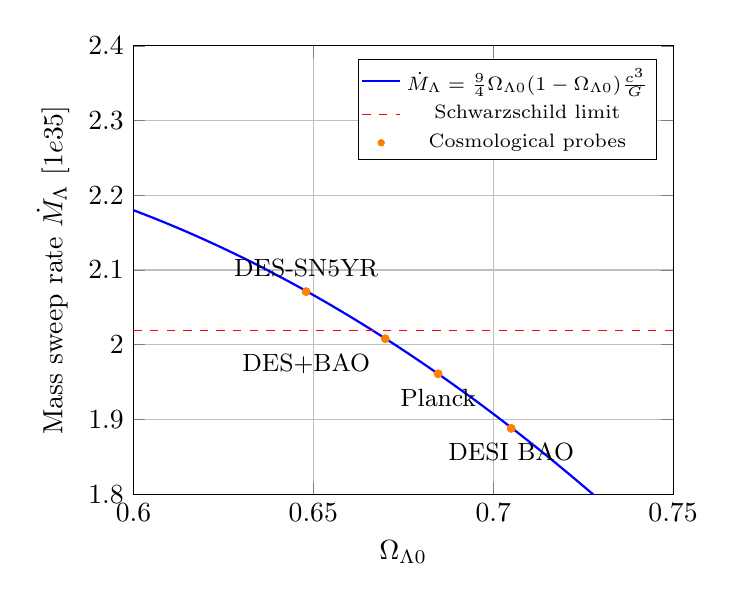
\begin{tikzpicture} \begin{axis}[ xlabel={$\Omega_{\Lambda0}$}, ylabel={Mass sweep rate $\dot{M}_\Lambda$ [$\SI{1e35}{\kilogram\per\second}$]}, xmin=0.60, xmax=0.75, ymin=1.8, ymax=2.4, xtick={0.60,0.65,0.70,0.75}, ytick={1.8,1.9,2.0,2.1,2.2,2.3,2.4}, legend pos=north east, legend style={font=\scriptsize, row sep=0pt, inner xsep=1pt, inner ysep=1pt}, legend image post style={xscale=0.8, yscale=0.8}, grid=major, ] \addplot[blue, thick, domain=0.60:0.75, samples=200] {(9/4) * x * (1 - x) * 4.037}; \addplot[red, dashed] coordinates {(0.60,2.019) (0.75,2.019)}; \addplot[only marks, mark=*, mark size=1.4, color=orange] coordinates {(0.648,2.071) (0.670,2.008) (0.6847,1.961) (0.705,1.888)}; \node at (axis cs:0.648,2.071) [above=2pt, font=\small] {DES-SN5YR}; \node at (axis cs:0.670,2.008) [below left=2pt, font=\small] {DES+BAO}; \node at (axis cs:0.6847,1.961) [below=2pt, font=\small] {Planck}; \node at (axis cs:0.705,1.888) [below=2pt, font=\small] {DESI BAO}; \legend{$\dot{M}_\Lambda = \frac{9}{4} \Omega_{\Lambda0} (1 - \Omega_{\Lambda0}) \frac{c^3}{G}$, Schwarzschild limit, Cosmological probes} \end{axis}
\end{tikzpicture}
\caption{Mass sweep rate $\dot{M}_\Lambda$ versus $\Omega_{\Lambda0}$. The blue curve shows $\dot{M}_\Lambda = \frac{9}{4} \Omega_{\Lambda0} (1 - \Omega_{\Lambda0}) \frac{c^3}{G}$ (with $c^3/2G = \SI{2.019e35}{\kilogram\per\second}$). The red dashed line is the Schwarzschild limit. Orange points mark recent probes.}
\label{fig:omega}
\end{figure}